%package list
\documentclass{article}
\usepackage[top=3cm, bottom=3cm, outer=3cm, inner=3cm]{geometry}
\usepackage{multicol}
\usepackage{graphicx}
\usepackage{url}
%\usepackage{cite}
\usepackage{hyperref}
\usepackage{array}
\usepackage{bookmark}
%\usepackage{multicol}
\newcolumntype{x}[1]{>{\centering\arraybackslash\hspace{0pt}}p{#1}}
\usepackage{natbib}
\usepackage{pdfpages}
\usepackage{multirow}
\usepackage[normalem]{ulem}
\useunder{\uline}{\ul}{}
\usepackage{xcolor}
\usepackage{listings}
\lstdefinestyle{ascii-tree}{
    literate={├}{|}1 {─}{--}1 {└}{+}1 
  }
\lstset{basicstyle=\ttfamily,
  showstringspaces=false,
  commentstyle=\color{red},
  keywordstyle=\color{blue}
}
%\usepackage{booktabs}
\usepackage[labelformat=empty]{caption}
\usepackage{subcaption}
\usepackage{float}
\usepackage{array}
\usepackage{minted}

\setminted{fontsize=\small,numbers=left,autogobble}
\newenvironment{block}{\captionsetup{type=listing}}{}

\newcolumntype{M}[1]{>{\centering\arraybackslash}m{#1}}
\newcolumntype{N}{@{}m{0pt}@{}}





%%%%%%%%%%%%%%%%%%%%%%%%%%%%%%%%%%%%%%%%%%%%%%%%%%%%%%%%%%%%%%%%%%%%%%%%%%%%
%%%%%%%%%%%%%%%%%%%%%%%%%%%%%%%%%%%%%%%%%%%%%%%%%%%%%%%%%%%%%%%%%%%%%%%%%%%%
\newcommand{\itemEmail}{cmestasz@unsa.edu.pe}
\newcommand{\itemStudent}{Christian Raul Mestas Zegarra}
\newcommand{\itemStudentShort}{Christian Mestas}
\newcommand{\itemCourse}{Programación Web 2}
\newcommand{\itemCourseCode}{1702122}
\newcommand{\itemSemester}{I}
\newcommand{\itemUniversity}{Universidad Nacional de San Agustín de Arequipa}
\newcommand{\itemFaculty}{Facultad de Ingeniería de Producción y Servicios}
\newcommand{\itemDepartment}{Departamento Académico de Ingeniería de Sistemas e Informática}
\newcommand{\itemSchool}{Escuela Profesional de Ingeniería de Sistemas}
\newcommand{\itemAcademic}{2023 - B}
\newcommand{\itemInput}{Del 24 Junio 2024}
\newcommand{\itemOutput}{Al 06 Julio 2024}
\newcommand{\itemPracticeNumber}{10}
\newcommand{\itemTheme}{Proyecto Final}
\renewcommand{\contentsname}{Laboratorio \itemPracticeNumber}
%%%%%%%%%%%%%%%%%%%%%%%%%%%%%%%%%%%%%%%%%%%%%%%%%%%%%%%%%%%%%%%%%%%%%%%%%%%%
%%%%%%%%%%%%%%%%%%%%%%%%%%%%%%%%%%%%%%%%%%%%%%%%%%%%%%%%%%%%%%%%%%%%%%%%%%%%

\usepackage[utf8]{inputenc}
\renewcommand{\figurename}{Figura}
\renewcommand{\refname}{Referencias}
\renewcommand{\tablename}{Tabla} %esto no funciona cuando se usa babel
\AtBeginDocument{%
\renewcommand\tablename{Tabla}
\setlength{\headheight}{40.51407pt}
}

\usepackage{fancyhdr}
\pagestyle{fancy}
\fancyhf{}
\setlength{\headheight}{30pt}
\renewcommand{\headrulewidth}{1pt}
\renewcommand{\footrulewidth}{1pt}
\fancyhead[L]{\raisebox{-0.2\height}{
\includegraphics[width=3cm]{img/logo_episunsa.png}}}
\fancyhead[C]{\fontsize{7}{7}\selectfont	\itemUniversity \\ \itemFaculty \\ \itemDepartment \\ \itemSchool \\ \textbf{\itemCourse}}
\fancyhead[R]{\raisebox{-0.2\height}{
\includegraphics[width=1.2cm]{img/logo_abet.png}}}
\fancyfoot[L]{\itemStudentShort}
\fancyfoot[C]{\itemCourse}
\fancyfoot[R]{Página \thepage}

% para el codigo fuente
\usepackage{listings}
\usepackage{color, colortbl}
\definecolor{dkgreen}{rgb}{0,0.6,0}
\definecolor{gray}{rgb}{0.5,0.5,0.5}
\definecolor{mauve}{rgb}{0.58,0,0.82}
\definecolor{codebackground}{rgb}{0.95, 0.95, 0.92}
\definecolor{tablebackground}{rgb}{0.8, 0, 0}

\begin{document}

\vspace*{10px}

\begin{center}
	\fontsize{17}{17} \textbf{ Informe de Laboratorio \itemPracticeNumber}
\end{center}
\centerline{\textbf{\Large Tema: \itemTheme}}
%\vspace*{0.5cm}	

\begin{flushright}
	\begin{tabular}{|M{2.5cm}|N|}
		\hline
		\rowcolor{tablebackground}
		\color{white} \textbf{Nota} \\
		\hline
		\\[30pt]
		\hline
	\end{tabular}
\end{flushright}

\begin{table}[H]
	\begin{tabular}{|M{5.4cm}|M{4.0cm}|M{4.7cm}|}
		\hline
		\rowcolor{tablebackground}
		\color{white} \textbf{Estudiante(s)} & \color{white}\textbf{Escuela} & \color{white}\textbf{Asignatura}                                        \\
		\hline
		{\itemStudent \par \itemEmail}       & \itemSchool                   & {\itemCourse \par Semestre: \itemSemester \par Código: \itemCourseCode} \\
		\hline
	\end{tabular}
\end{table}

\begin{table}[H]
	\begin{tabular}{|M{4.7cm}|M{4.7cm}|M{4.7cm}|}
		\hline
		\rowcolor{tablebackground}
		\color{white}\textbf{Laboratorio} & \color{white}\textbf{Tema} & \color{white}\textbf{Duración} \\
		\hline
		\itemPracticeNumber               & \itemTheme                 & 04 horas                       \\
		\hline
	\end{tabular}
\end{table}

\begin{table}[H]
	\begin{tabular}{|M{4.7cm}|M{4.7cm}|M{4.7cm}|}
		\hline
		\rowcolor{tablebackground}
		\color{white}\textbf{Semestre académico} & \color{white}\textbf{Fecha de inicio} & \color{white}\textbf{Fecha de entrega} \\
		\hline
		\itemAcademic                            & \itemInput                            & \itemOutput                            \\
		\hline
	\end{tabular}
\end{table}
\pagebreak

\tableofcontents
\pagebreak


%%%%%%%%%%%%%%%%%%%%%%%%%%%%%%%%%%%%%%%%%%%%%%%%%%%%%%%%%%%%%%%%%%%%%%
\section{Tarea}
\begin{itemize}
	\item \textbf{Enunciado:}
	      \begin{itemize}
		      \item Este trabajo debe ser hecho en grupos de 3 a 4. Escoger una empresa, escoger el tema a trabajar y definir los Requerimientos funcionales.
		      \item El trabajo en equipo, debe ser hecho de modo que todos los participantes del grupo conozcan todo el código.
		            \begin{itemize}
			            \item La programación debe ser hecha en pares, es decir que durante una videollamada, dos o más integrantes (al menos dos, pueden ser todos los integrantes del grupo) programen un mismo código en un repositorio central, turnándose la labor de observador y codificar a intervalos de tiempo equitativos.
			            \item No se debe dividir el trabajo en partes y que los integrantes hagan su parte sin que los demás conozcan de su trabajo o él conozca y participe en el trabajo de los demás.
			            \item Se deben crear ramas en sus proyectos de git para cada una de las funcionalidades, una vez alcanzada con éxito la funcionalidad, esta se debe integrar a la rama principal.
		            \end{itemize}
		      \item La aplicación será calificada sobre 20 y deberá incluir:
		            \begin{itemize}
			            \item URLs propios, usando reverse (2 puntos)
			            \item Plantillas propias de la aplicación (1 puntos)
			            \item Que usen widgets de manera elegante (1 puntos)
			            \item Vistas de Listado, Detalle, Crear, Actualizar y Borrar (4 puntos)
			            \item Formulario con restricciones de seguridad adicionales (2 puntos)
			            \item Vista de consultas que devuelva Json (3 puntos)
			            \item Programa cliente para hacer y consumir las consultas con Ajax (2 puntos)
			            \item Programa cliente para hacer y consumir las consultas con Framework de JavaScript (3 puntos)
			            \item Al menos dos modelos (2 puntos)
			            \item Modelo con clave externa: foreign key (+2 puntos, opcional)
			            \item CSS o Bootstrap (2 puntos)
			            \item Publicó su aplicación en el web (+3 puntos, opcional)
			            \item Descargar un informe como archivos pdf (+2 puntos, opcional)
			            \item Enviar correo (+2 puntos, opcional)
		            \end{itemize}
		      \item Trabajo en equipo, los 20 puntos serán distribuidos de manera equitativa entre los siguientes criterios
		            \begin{itemize}
			            \item Responsabilidad: cumplió puntualmente con todo
			            \item Proactividad: hizo más de lo que se pidió
			            \item Aporte al grupo
			            \item Calificó a sus compañeros (Si no lo hizo 50\% de la nota de trabajo individual)
		            \end{itemize}
		      \item La calificación final será un promedio entre la nota individual 40\% y grupal 60\%
		            \begin{itemize}
			            \item La nota grupal será por el producto calificado por el profesor, en base a sus avances, exposición e informe.
			            \item La nota individual será calificada por sus propios compañeros. Los que no califiquen a sus compañeros tendrán la mitad de la nota en este componente.
		            \end{itemize}
	      \end{itemize}
\end{itemize}
\pagebreak
%%%%%%%%%%%%%%%%%%%%%%%%%%%%%%%%%%%%%%%%%%%%%%%%%%%%%%%%%%%%%%%%%%%%%%

\section{Equipos y materiales utilizados}
\begin{itemize}
	%%%%%%%%%%%%%%%%%%%%%%%%%%%%%%%%%%%%%%%%%%%%%%%%%%%%%%%%%%%%%%%%%%%%%%
	\item Cuenta en GitHub con el correo institucional.
	\item Sistema Operativo Microsoft Windows 10
	\item Visual Studio Code
	\item Git
	\item Windows PowerShell
	\item Navegador Mozilla Firefox
	\item Angular CLI
	\item Django
	      %%%%%%%%%%%%%%%%%%%%%%%%%%%%%%%%%%%%%%%%%%%%%%%%%%%%%%%%%%%%%%%%%%%%%%
\end{itemize}
\pagebreak

\section{Desarrollo}
\subsection{Backend en Django}
\begin{block}
	\caption{models.py}
	\inputminted[breaklines]{Python}{kioskios_api/api/models.py}
	\begin{itemize}
		\item Se crean los modelos \textbf{Usuario}, \textbf{Tienda}, \textbf{Producto} y \textbf{Venta}.
		\item Se crea la clase \textbf{UsuarioManager} para poder usar la autenticación de Django.
	\end{itemize}

	\caption{forms.py}
	\inputminted{Python}{kioskios_api/api/forms.py}
	\begin{itemize}
		\item Se crean los formularios \textbf{UsuarioForm}, \textbf{DueñoForm}, \textbf{AdminForm}, \textbf{TiendaForm}, \textbf{ProductoForm} y \textbf{VentaForm}.
		\item Además se crean los formularios \textbf{LoginForm} y \textbf{LogoutForm} para el inicio y cierre de sesión.
		\item Los formularios tienen validaciones personalizadas para los campos.
	\end{itemize}

	\caption{serializers.py}
	\inputminted[breaklines]{Python}{kioskios_api/api/serializers.py}
	\begin{itemize}
		\item Se crea el serializador para formularios, que puede convertir todos los campos del formulario en un JSON.
		\item Se crea el serializador para los modelos, que puede convertir todos los campos del modelo en un JSON.
	\end{itemize}

	\caption{decorators.py}
	\inputminted{Python}{kioskios_api/api/decorators.py}
	\begin{itemize}
		\item Se crea el decorador \textbf{api\_login\_required} para verificar si el usuario está autenticado al hacer las peticiones por api.
	\end{itemize}

	\caption{views.py}
	\inputminted[breaklines]{Python}{kioskios_api/api/views.py}
	\begin{itemize}
		\item Se crean las vistas para los formularios de \textbf{Usuario}, \textbf{Dueño}, \textbf{Admin}, \textbf{Tienda}, \textbf{Producto} y \textbf{Venta}.
		\item También se crean las vistas para obtener los listados de los modelos de acuerdo al nivel de acceso.
		\item Estas vistas retornan un JSON con los datos del formulario tras ser serializados y reciben las respuestas del form.
		\item Se crean las vistas \textbf{iniciar\_sesion} y \textbf{cerrar\_sesion} para el inicio y cierre de sesión.
	\end{itemize}

	\caption{urls.py}
	\inputminted{Python}{kioskios_api/api/urls.py}
	\begin{itemize}
		\item Se crean las rutas para las vistas de los formularios y los listados de los modelos.
		\item Se crean las rutas para las vistas de inicio y cierre de sesión.
	\end{itemize}
\end{block}
\pagebreak

\subsection{Frontend en Angular}
\subsubsection{Aplicación base}
\begin{block}
	\caption{app.routes.ts}
	\inputminted{TypeScript}{kioskios_web/src/app/app.routes.ts}
	\begin{itemize}
		\item Archivo de rutas de la aplicación.
		\item Se crean las rutas para los componentes \textbf{home}, \textbf{login} y \textbf{register}.
	\end{itemize}

	\caption{styles.css}
	\inputminted{CSS}{kioskios_web/src/styles.css}
	\begin{itemize}
		\item Estilos de la aplicación.
		\item Se encarga de dar estilos generales a la aplicación.
	\end{itemize}
\end{block}

\subsubsection{dynamic-form}
\begin{block}
	\caption{loader-form.component.ts}
	\inputminted{TypeScript}{kioskios_web/src/app/dinamic-form/loader-form/loader-form.component.ts}
	\begin{itemize}
		\item Componente que se encarga de cargar el formulario dinámico.
		\item Se encarga de recibir los datos del formulario y enviarlos al componente \textbf{dynamic-form}.
	\end{itemize}

	\caption{dynamic-form.component.ts}
	\inputminted[breaklines]{TypeScript}{kioskios_web/src/app/dinamic-form/dinamic-form.component.ts}
	\begin{itemize}
		\item Componente que se encarga de crear un formulario dinámico.
		\item Recibe un JSON con los campos del formulario y se encarga de deserializar los datos enviados desde Django.
	\end{itemize}

	\caption{dynamic-form.component.html}
	\inputminted[breaklines]{HTML}{kioskios_web/src/app/dinamic-form/dinamic-form.component.html}
	\begin{itemize}
		\item Plantilla del componente \textbf{dynamic-form}.
		\item Se crean los campos del formulario de acuerdo al JSON recibido.
	\end{itemize}
\end{block}

\subsubsection{home}
\begin{block}
	\caption{footer.component.ts}
	\inputminted[breaklines]{TypeScript}{kioskios_web/src/app/home/footer/footer.component.ts}
	\begin{itemize}
		\item Componente que se encarga de mostrar el footer de la página.
	\end{itemize}

	\caption[breaklines]{header.component.ts}
	\inputminted{TypeScript}{kioskios_web/src/app/home/header/header.component.ts}
	\begin{itemize}
		\item Componente que se encarga de mostrar el header de la página.
	\end{itemize}

	\caption[breaklines]{nav.component.ts}
	\inputminted{TypeScript}{kioskios_web/src/app/home/nav/nav.component.ts}
	\begin{itemize}
		\item Componente que se encarga de mostrar la barra de navegación de la página.
	\end{itemize}

	\caption[breaklines]{banner.component.ts}
	\inputminted{TypeScript}{kioskios_web/src/app/home/banner/banner.component.ts}
	\begin{itemize}
		\item Componente que se encarga de mostrar el banner de la página.
	\end{itemize}

	\caption{home.component.ts}
	\inputminted{TypeScript}{kioskios_web/src/app/home/home.component.ts}
	\begin{itemize}
		\item Componente que se encarga de mostrar la página principal.
		\item Posee redirecciones a las demás páginas de la aplicación.
	\end{itemize}

	\caption{home.component.html}
	\inputminted{HTML}{kioskios_web/src/app/home/home.component.html}
	\begin{itemize}
		\item Plantilla del componente \textbf{home}.
		\item Se muestran los componentes \textbf{header}, \textbf{nav} y \textbf{footer}.
	\end{itemize}
\end{block}

\subsubsection{login}
\begin{block}
	\caption{login.component.ts}
	\inputminted{TypeScript}{kioskios_web/src/app/login/login.component.ts}
	\begin{itemize}
		\item Componente que se encarga de mostrar el formulario de inicio de sesión.
		\item Se encarga de enviar los datos al backend y recibir la respuesta.
	\end{itemize}

	\caption{login.component.html}
	\inputminted{HTML}{kioskios_web/src/app/login/login.component.html}
	\begin{itemize}
		\item Plantilla del componente \textbf{login}.
		\item Se muestra el formulario de inicio de sesión.
	\end{itemize}
\end{block}

\subsubsection{register}
\begin{block}
	\caption{register.component.ts}
	\inputminted{TypeScript}{kioskios_web/src/app/register/register.component.ts}
	\begin{itemize}
		\item Componente que se encarga de mostrar el formulario de registro.
		\item Se encarga de enviar los datos al backend y recibir la respuesta.
	\end{itemize}

	\caption{register.component.html}
	\inputminted{HTML}{kioskios_web/src/app/register/register.component.html}
	\begin{itemize}
		\item Plantilla del componente \textbf{register}.
		\item Se muestra el formulario de registro.
	\end{itemize}

	\caption{register.component.css}
	\inputminted{CSS}{kioskios_web/src/app/register/register.component.css}
	\begin{itemize}
		\item Estilos del componente \textbf{register}.
		\item Se encarga de dar estilos al formulario de registro.
	\end{itemize}
\end{block}

\subsubsection{services}
\begin{block}
	\caption{api.service.ts}
	\inputminted{TypeScript}{kioskios_web/src/app/services/api.service.ts}
	\begin{itemize}
		\item Servicio que se encarga de realizar las peticiones al backend.
		\item Se encarga de enviar los datos al backend y recibir la respuesta.
	\end{itemize}

	\caption{auth-interceptor.service.ts}
	\inputminted[breaklines]{TypeScript}{kioskios_web/src/app/services/auth-interceptor.service.ts}
	\begin{itemize}
		\item Servicio que se encarga de interceptar las peticiones al backend.
		\item Se encarga de enviar el token de autenticación en las peticiones.
	\end{itemize}
\end{block}

\subsubsection{models}
\begin{block}
	\caption{form-field.ts}
	\inputminted{TypeScript}{kioskios_web/src/app/models/form-field.ts}
	\begin{itemize}
		\item Modelo que se encarga de definir los campos de un formulario.
		\item Usado para la creación de formularios dinámicos.
	\end{itemize}
\end{block}
\pagebreak


\subsection{Demostración}
\begin{block}
	\centering
	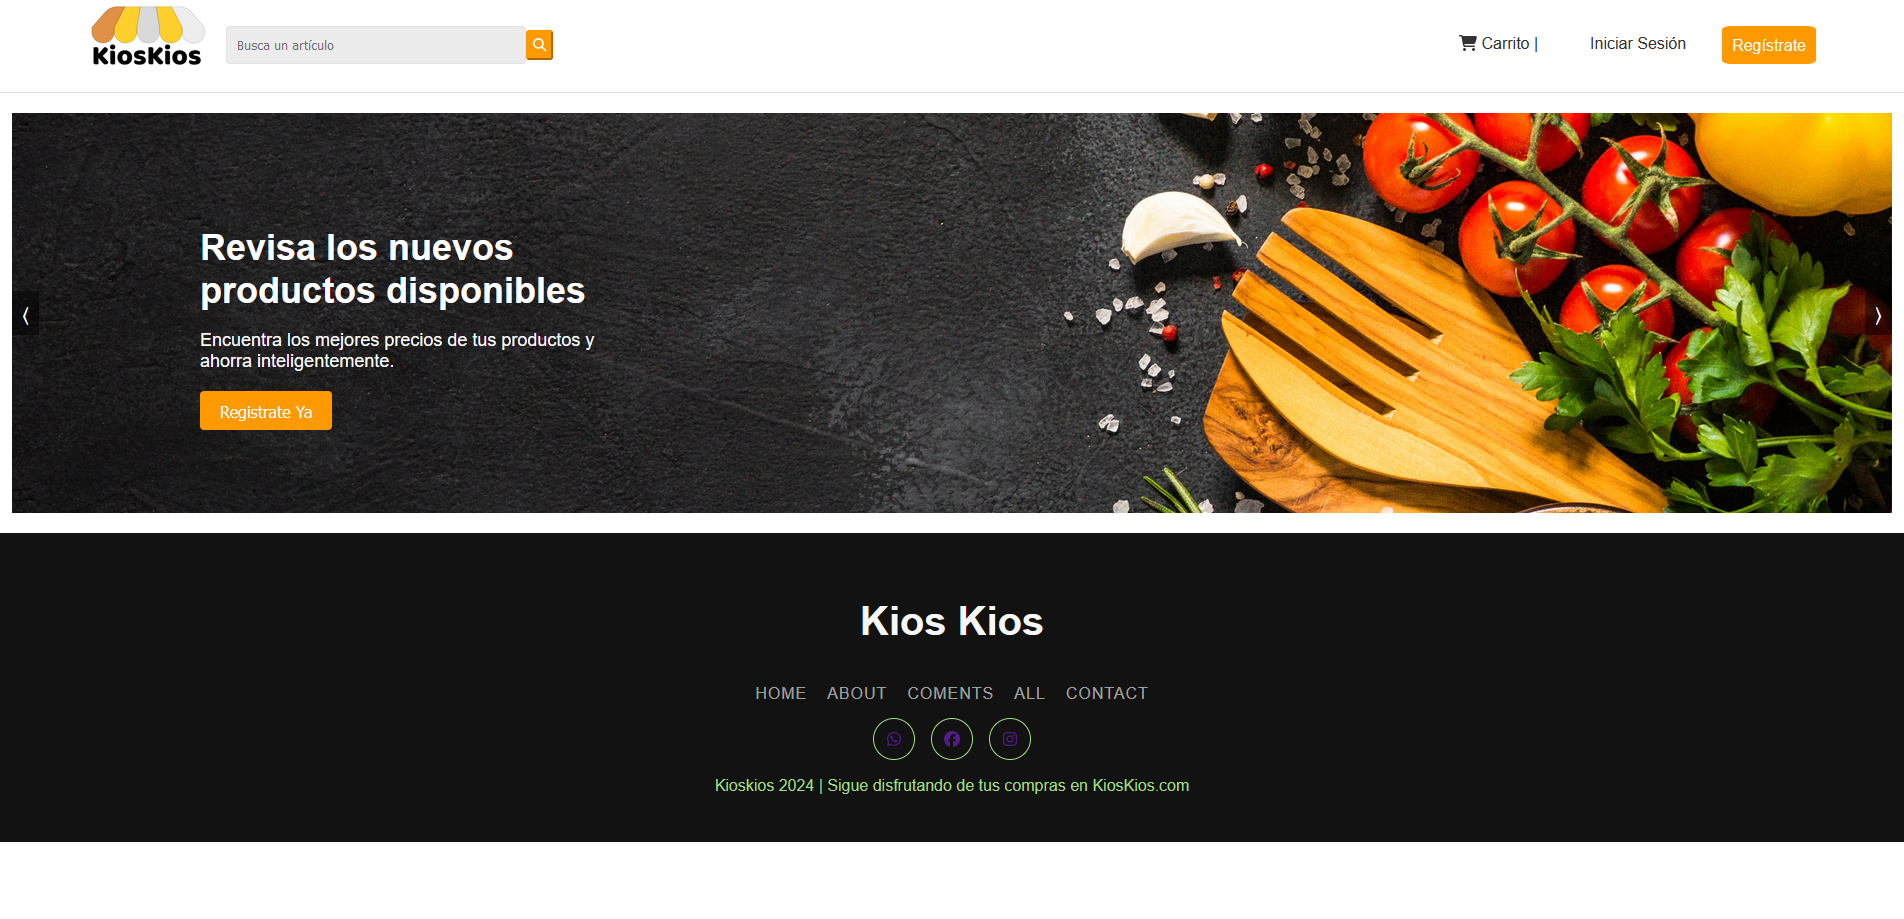
\includegraphics[width=0.8\textwidth]{img/E1.png}
	\caption{Página principal.}
	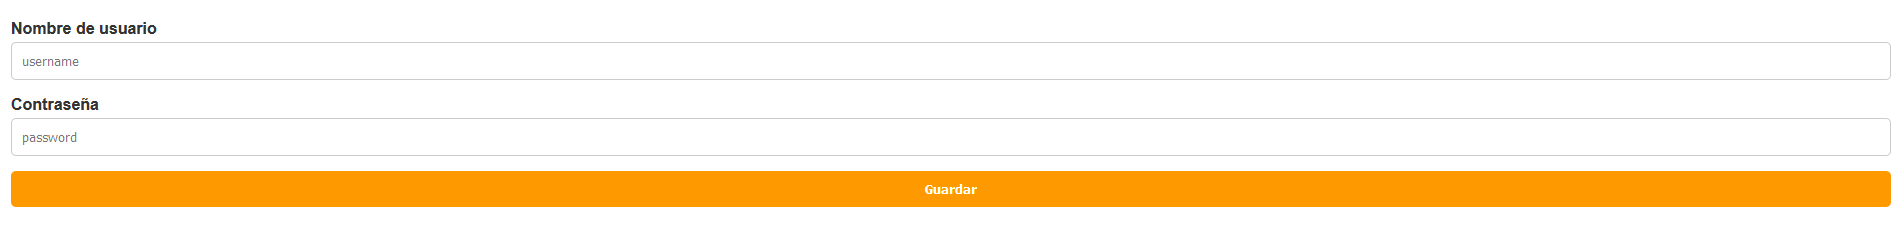
\includegraphics[width=0.8\textwidth]{img/E2.png}
	\caption{Inicio de sesión.}
	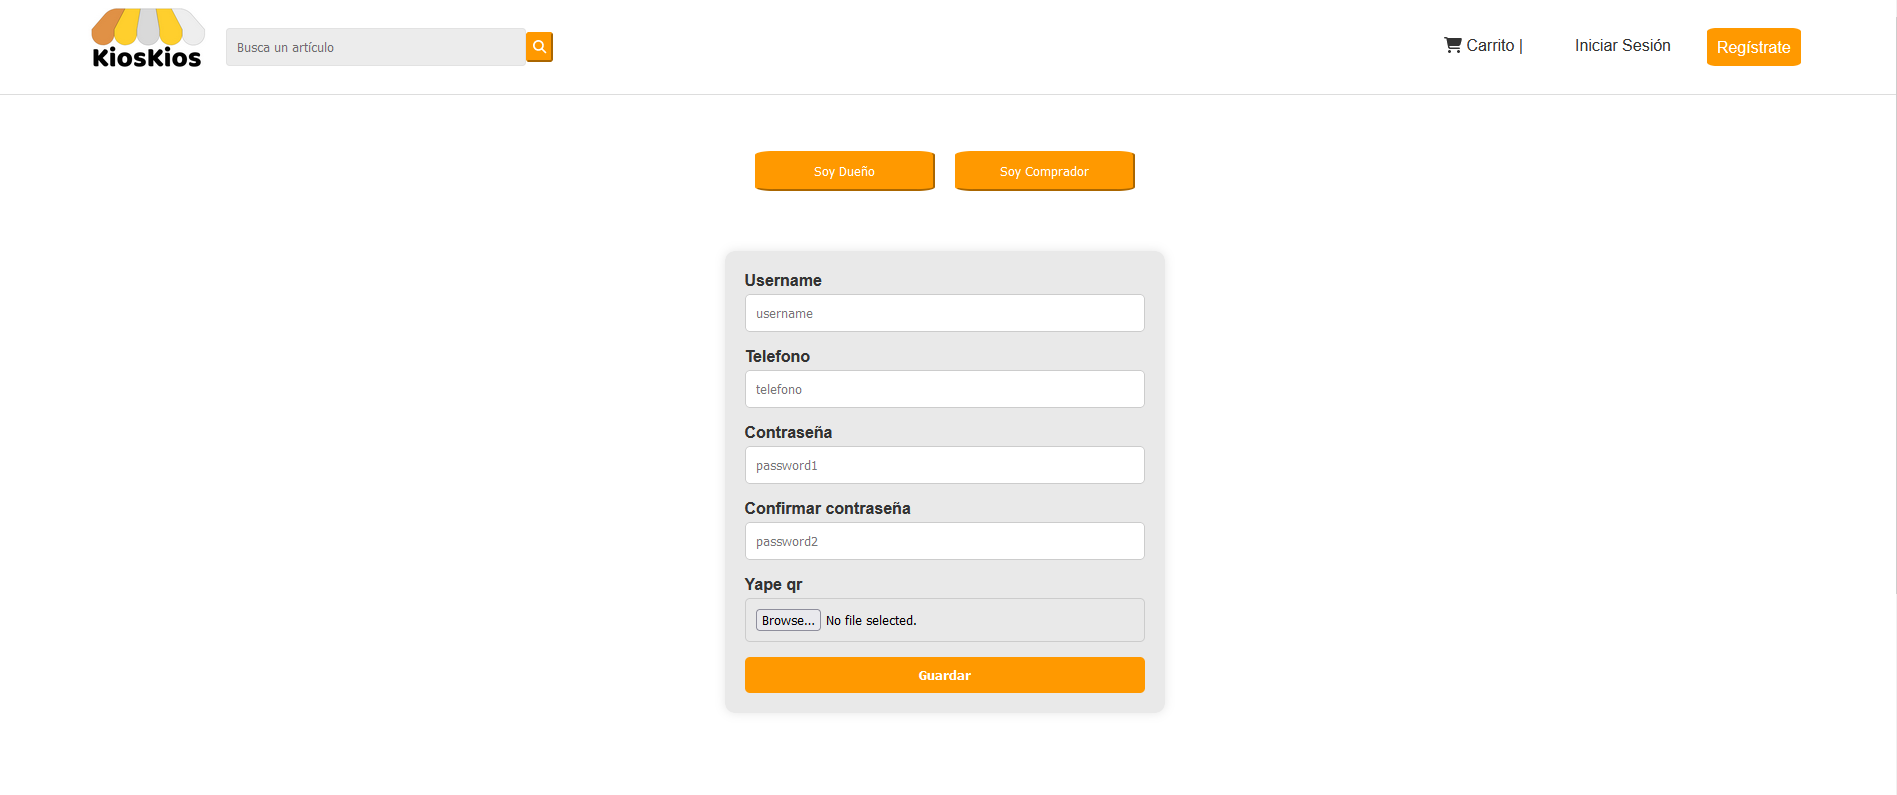
\includegraphics[width=0.8\textwidth]{img/E3.png}
	\caption{Registro.}
\end{block}
\pagebreak

\subsection{Lista de commits}
\begin{figure}[H]
	\centering
	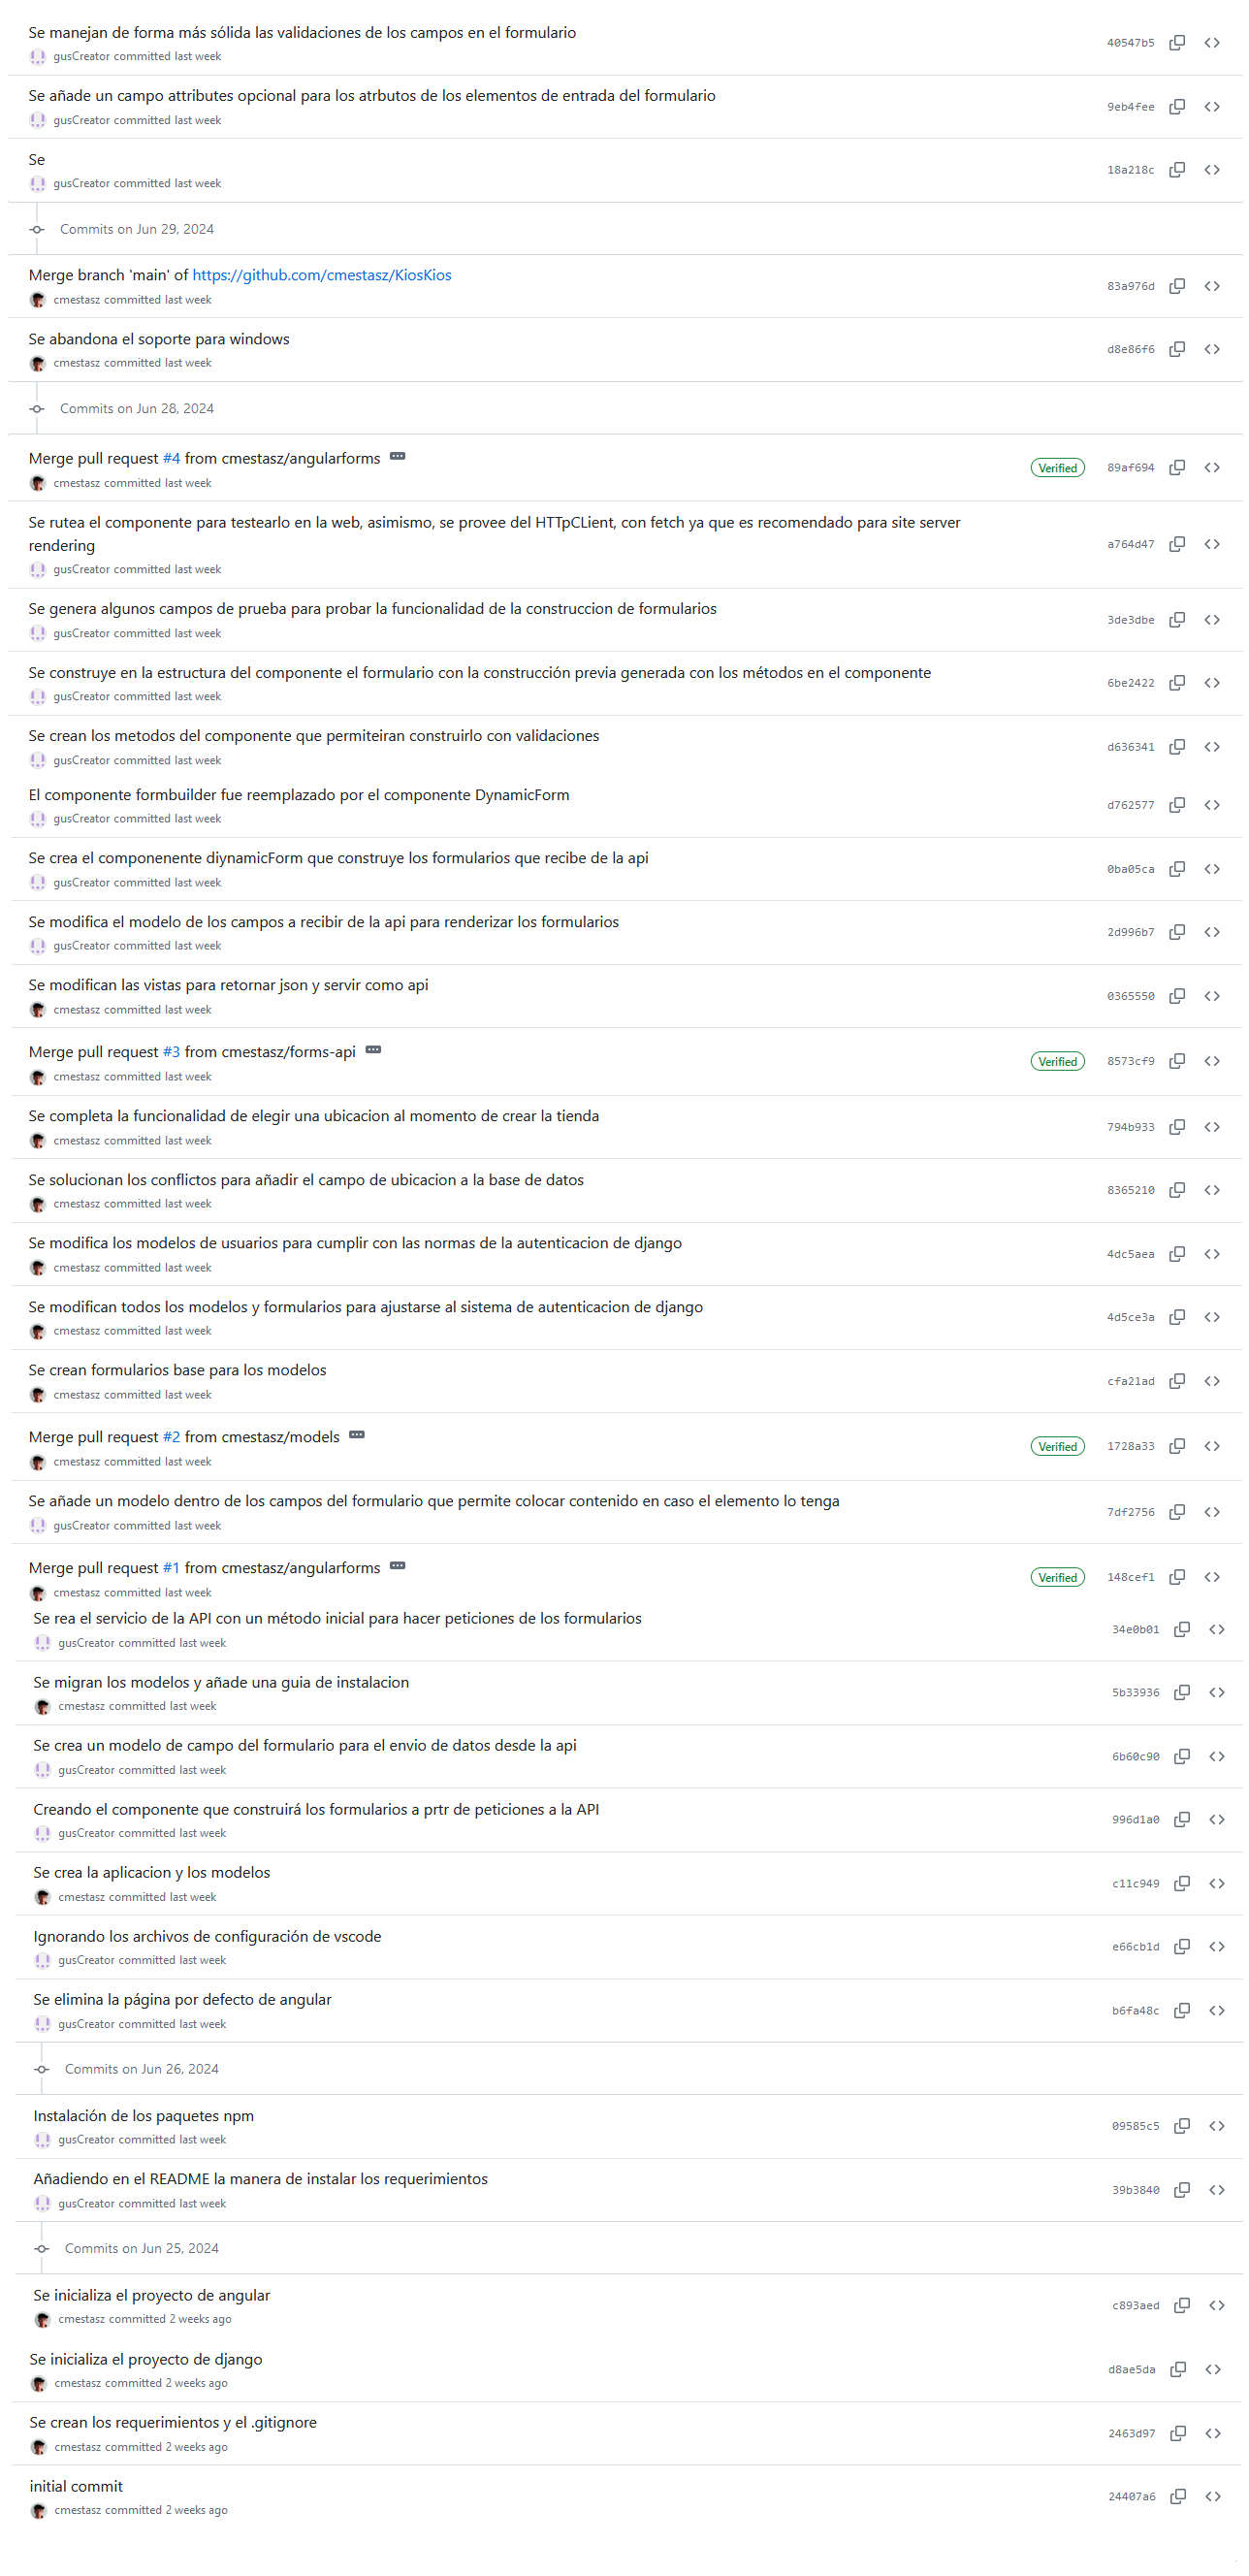
\includegraphics[width=0.5\textwidth,keepaspectratio]{img/commits1.png}
	\caption{Lista de commits.}
\end{figure}
\pagebreak
\begin{figure}[H]
	\centering
	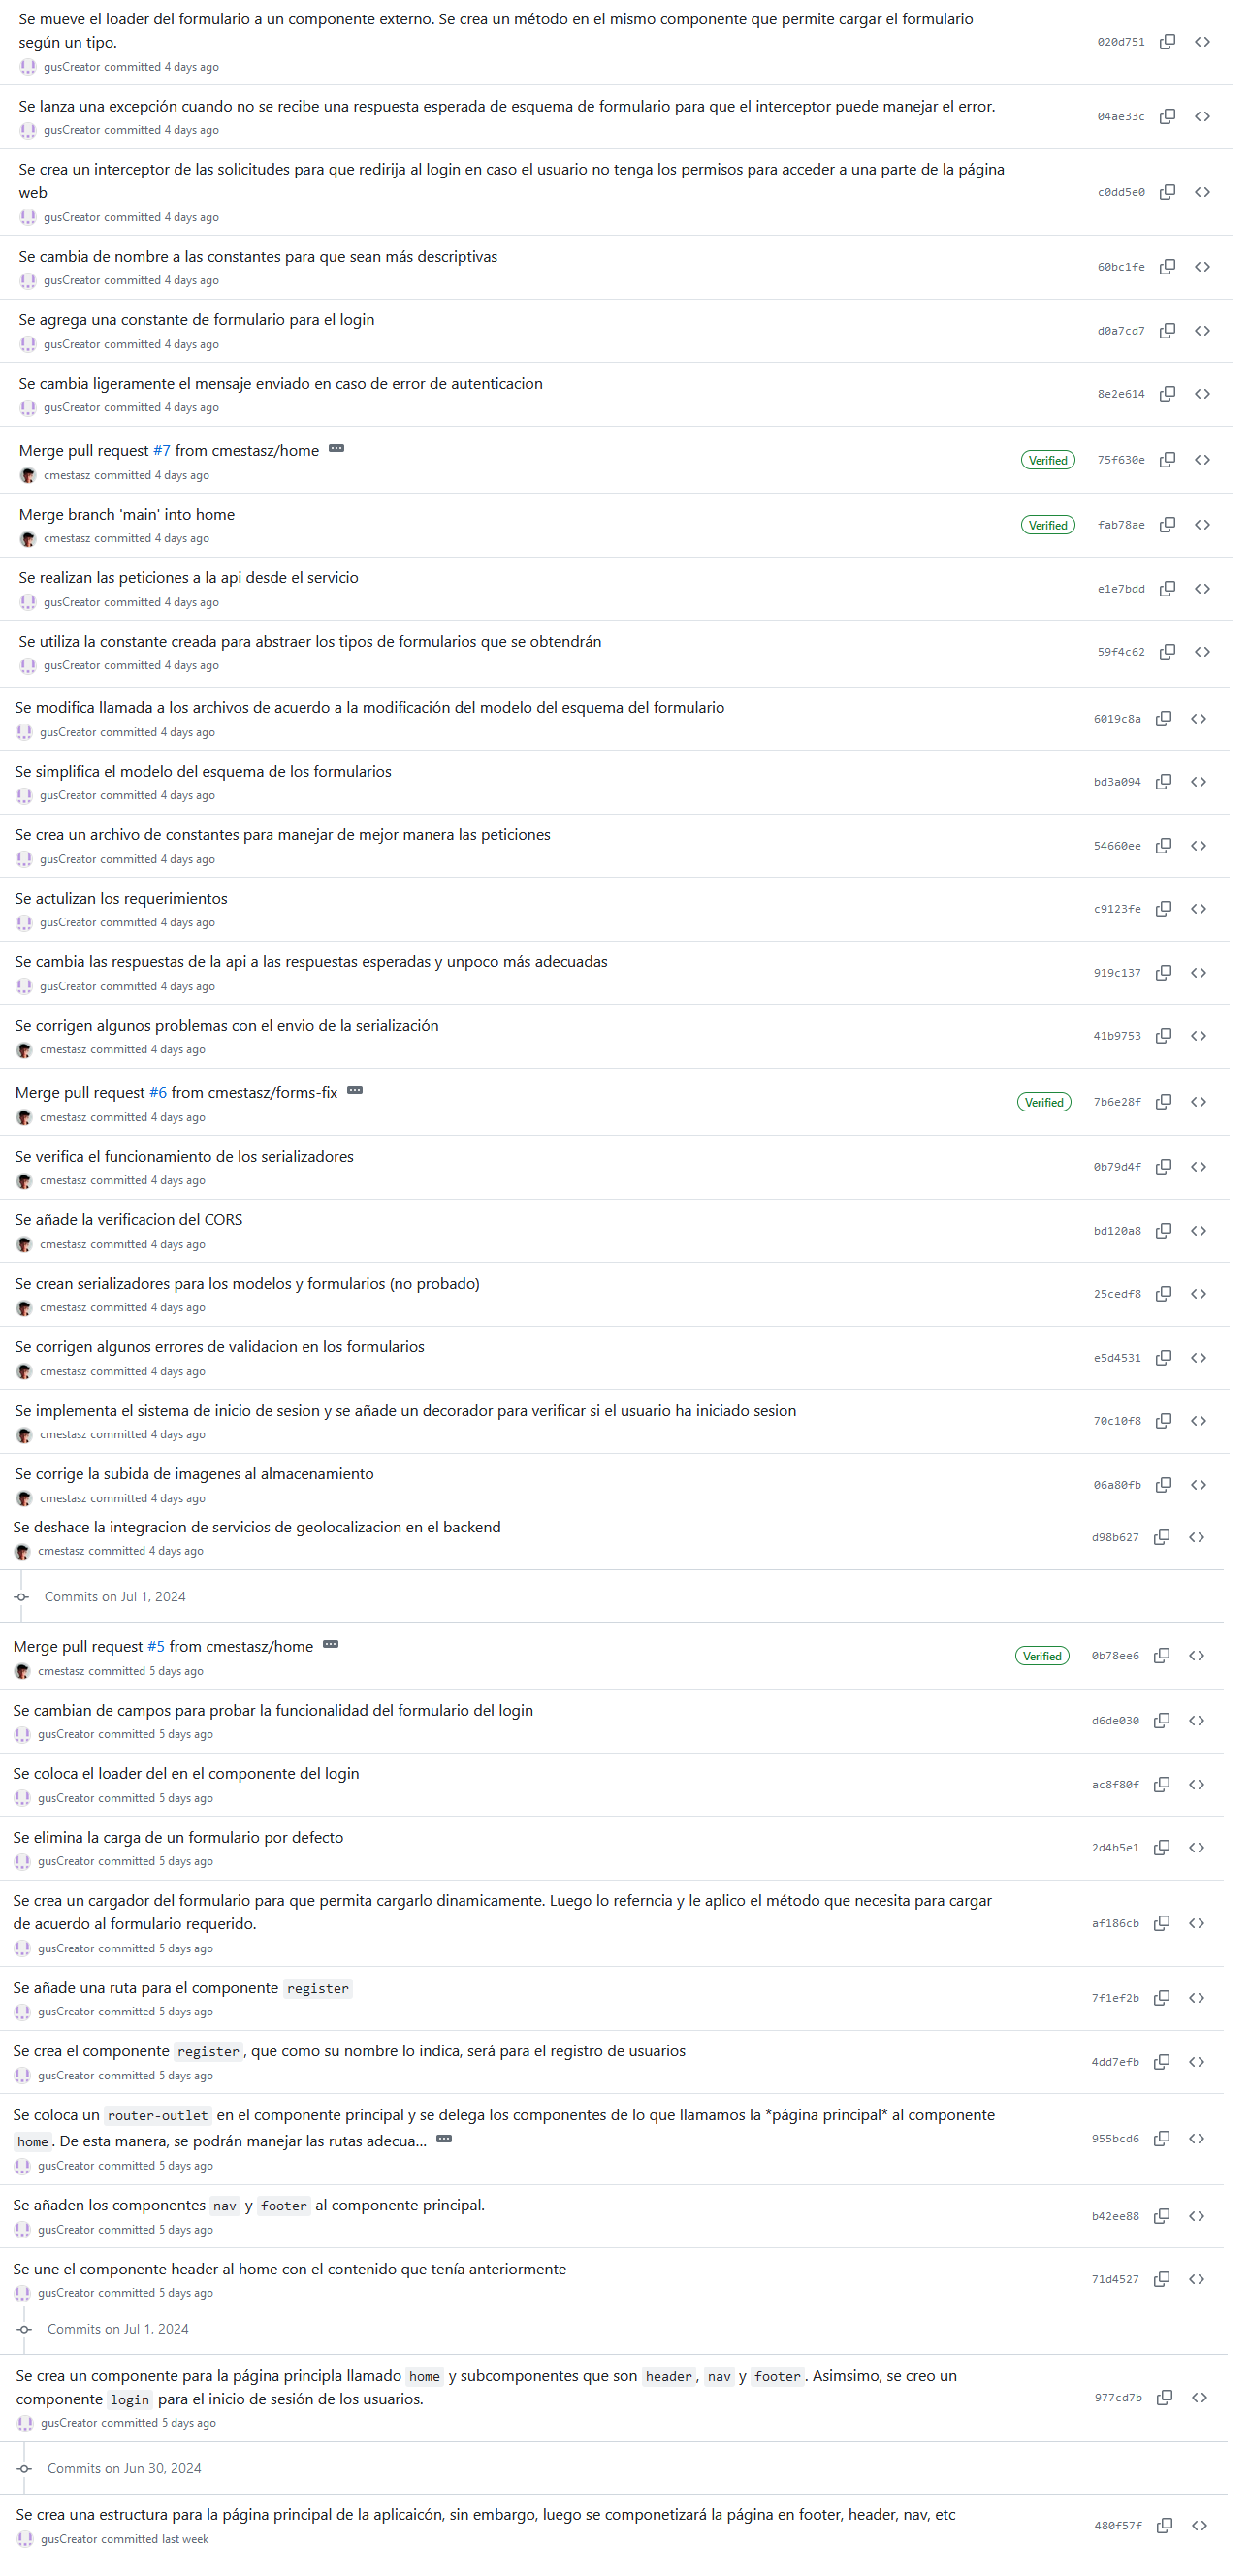
\includegraphics[width=0.5\textwidth,keepaspectratio]{img/commits2.png}
	\caption{Lista de commits.}
\end{figure}
\pagebreak
\begin{figure}[H]
	\centering
	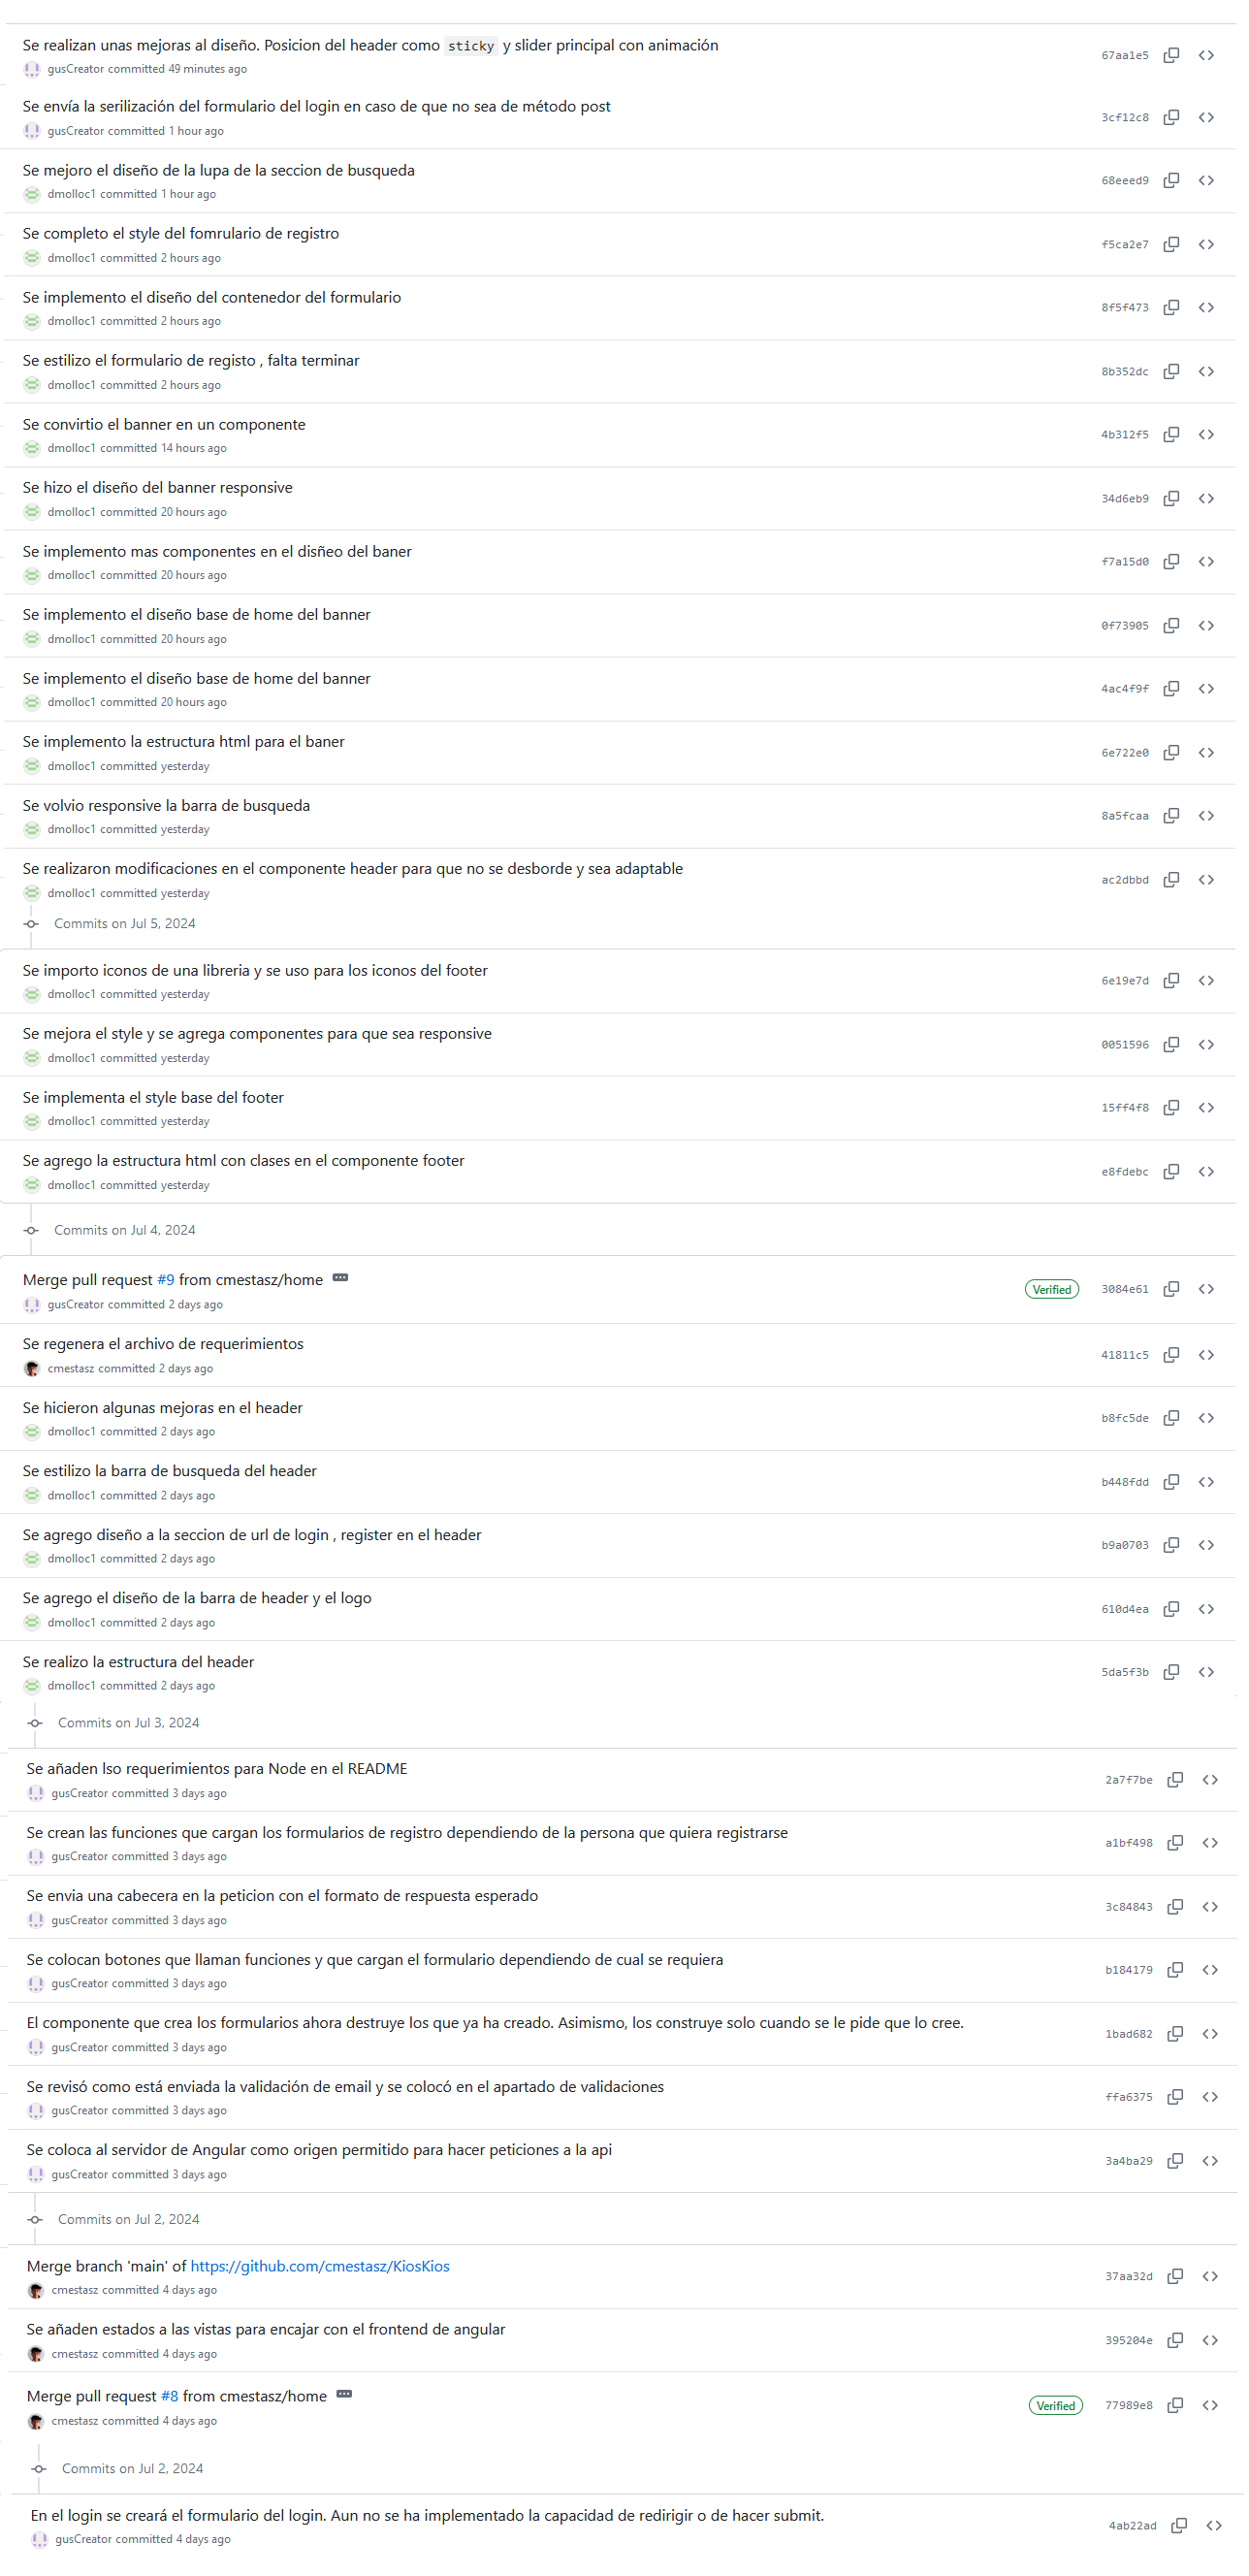
\includegraphics[width=0.5\textwidth,keepaspectratio]{img/commits3.png}
	\caption{Lista de commits.}
\end{figure}
\pagebreak
\pagebreak

\section{URL del repositorio en GitHub}
\begin{itemize}
	\item \url{https://github.com/cmestasz/KiosKios.git}
\end{itemize}

\section{Enlace al video}
\begin{itemize}
	\item \url{https://youtu.be/uV5e1j8fDv0}
\end{itemize}

\section{Estructura de laboratorio \itemPracticeNumber}
El contenido que se entrega en este laboratorio es el siguiente:
%%%%%%%%%%%%%%%%%%%%%%%%%%%%%%%%%%%%%%%%%%%%%%%%%%%%%%%%%%%%%%%%%%%%%%
\begin{minted}{bash}
KiosKios/
|--- Informe.pdf
|--- Informe.tex
|--- README.md
|--- kioskios_api
	|--- api
		|--- __init__.py
		|--- admin.py
		|--- apps.py
		|--- decorators.py
		|--- forms.py
		|--- migrations
		|--- models.py
		|--- serializers.py
		|--- tests.py
		|--- urls.py
		|--- views.py
	|--- kioskios_api
		|--- __init__.py
		|--- settings.py
		|--- urls.py
		|--- wsgi.py
	|--- manage.py
|--- kioskios_web
	|--- src
		|--- app
			|--- app.routes.ts
			|--- app.component.html
			|--- app.component.css
			|--- dinamic-form
				|--- loader-form
					|--- loader-form.component.ts
				|--- dynamic-form
					|--- dynamic-form.component.ts
					|--- dynamic-form.component.html
					|--- dynamic-form.component.spec.ts
					|--- dynamic-form.component.css
			|--- home
				|--- footer
					|--- footer.component.ts
				|--- header
					|--- header.component.ts
				|--- nav
					|--- nav.component.ts
				|--- banner
					|--- banner.component.ts
				|--- home.component.ts
				|--- home.component.html
				|--- home.component.css
			|--- login
				|--- login.component.ts
				|--- login.component.html
				|--- login.component.css
			|--- register
				|--- register.component.ts
				|--- register.component.html
				|--- register.component.css
			|--- services
				|--- api.service.ts
				|--- auth-interceptor.service.ts
			|--- models
				|--- form-field.ts
			|--- (otros archivos de configuración)
		|--- index.html
		|--- styles.css
		|--- main.ts
		|--- main.server.ts
	|--- (otros archivos de configuración)
|--- img
	|--- logo_abet.png
	|--- logo_episunsa.png
	|--- logo_unsa.jpg
	|--- E1.png
	|--- E2.png
	|--- E3.png
	|--- commits1.png
	|--- commits2.png
	|--- commits3.png
\end{minted}
%%%%%%%%%%%%%%%%%%%%%%%%%%%%%%%%%%%%%%%%%%%%%%%%%%%%%%%%%%%%%%%%%%%%%%

\section{Referencias}
\begin{itemize}
	\item \url{https://angular.dev/tutorials/learn-angular}
	\item \url{https://www.djangoproject.com/}
\end{itemize}

%\pagebreak
%\bibliographystyle{apalike}
%\bibliographystyle{IEEEtranN}
%\bibliography{bibliography}

\end{document}